При ненулевом $\delta$ распределение тёмной материи является нетермальным.
\begin{figure}[!h]
	\centering
	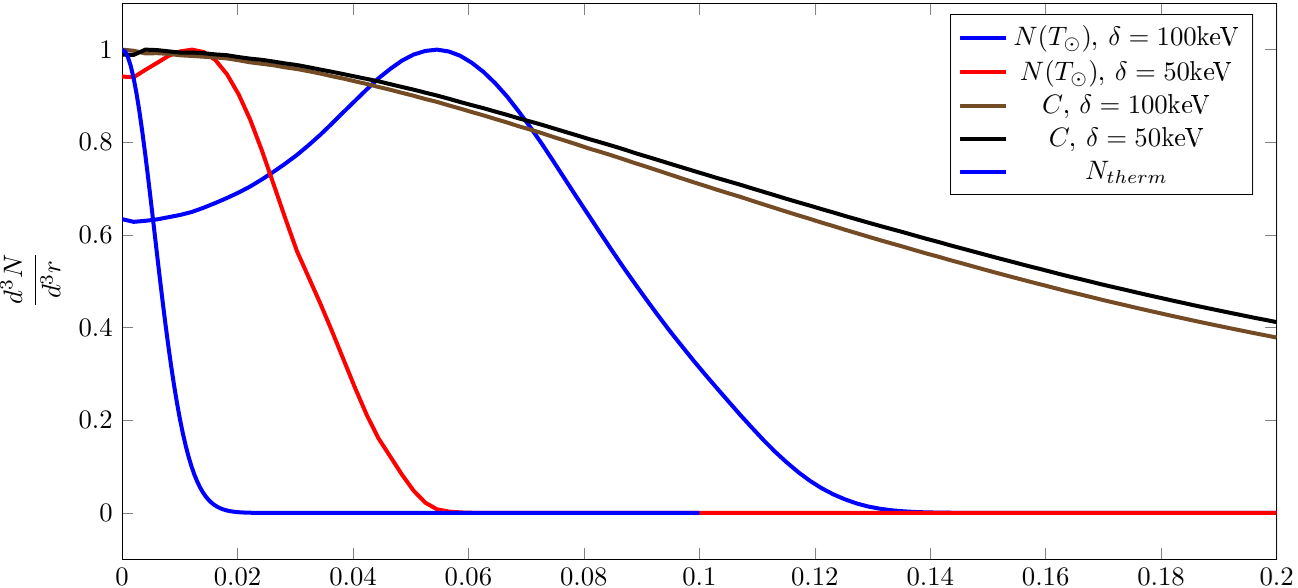
\includegraphics[width=0.8\textwidth]{images/Rdistribs.png}
	\caption{Начальное и конечное радиальное распределение частиц тёмной материи в Солнце $m_{\chi} = 100\text{GeV}$}
	\label{plot:Nrdistrib}
\end{figure}
